\documentclass[]{article}
\usepackage{tikz}
\usepackage{amsmath}
\usepackage{amssymb}
\usepackage{pgfplots}
\pgfplotsset{width=7cm,compat=1.8}
\usepgfplotslibrary{polar}

% Title Page
\title{%
	Complex Variables \\
	\large Week 1: \\
	Introduction to Complex Numbers}
\author{Nichole}
\date{August 25, 2018}


\begin{document}
\maketitle

\section{What is a Complex Number?}
	The encounter with complex numbers is usually presented as a solution to the equation: $\; x^2 = -1 \implies x=\pm\sqrt{-1}$    \\*
	
	\noindent Though this is an intuitive approach for a high school algebra class, it can be misleading. Consider the following: \\* 
	
	\indent \indent $i=\sqrt{-1}=\frac{\sqrt{-1}}{1}=\frac{\sqrt{-1}}{\sqrt{1}}=\sqrt{\frac{-1}{1}}=\sqrt{\frac{1}{-1}}=\frac{1}{i}$
	
	\indent \indent $\therefore i=\frac{1}{i} \; ? $ \\* 
	
	\noindent As you can see from this example, the imaginary number $i$ has properties that are different from real numbers.
	
	\subsection{A Better Definition}
	The complex field $\mathbb{C}$ is the set of ordered pairs of real numbers $(a,b)$ with the following properties: \\* 
	
	\indent \indent Addition: $\; (a,b)+(c,d)=(a+c,b+d)$ \\ 
	\indent \indent Multiplication: $\; (a,b)(c,d)=(ac-bd,ad+bc)$ \\ 
	
	\noindent With this definition, we can now consider the ordered pair $(0,1)$ which we will call $i$. If we multiply $i$ by itself: \\
	
	\indent \indent $(0,1)(0,1)=(-1,0)=-1$ \\* 
	
	\noindent ... we can conclude that $i=\sqrt{-1}$.
	
	\subsection{Notation}
	    The most common way to represent complex numbers is: $z=(x,y)=x+iy$ \\*    
	    \noindent \textbf{ALL} complex numbers can (and should) be written in this form. \\* 
	    
	    \noindent There are three graphical ways to represent complex numbers. First, they can be represented as points on a 2D plane: \\* 
	    
	    \begin{figure}[!h]
	    	\centering
	        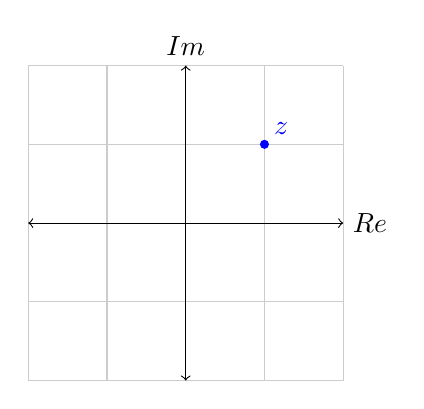
\begin{tikzpicture}
	            \draw[thin,gray!40] (-2,-2) grid (2,2);
	            \draw[<->] (-2,0)--(2,0) node[right]{$Re$}; % Horizontal Axis
	            \draw[<->] (0,-2)--(0,2) node[above]{$Im$}; % Vertical Axis
                \foreach \Point/\PointLabel in {(1,1)/z}    % Points
                \draw[fill=blue,blue] \Point circle (0.05) node[above right] {$\PointLabel$};
      	    \end{tikzpicture}
      	    \caption{The point $z=(1,1)=1+i$}
      	\end{figure}
	    
	    \noindent Secondly, complex numbers can also be represented as vectors beginning at the origin.
	    \begin{figure}[!h]
	    	\centering
            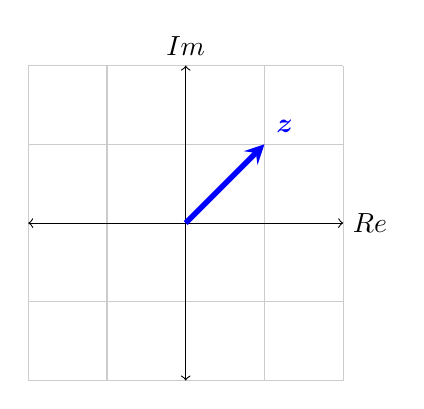
\begin{tikzpicture}
                \draw[thin,gray!40] (-2,-2) grid (2,2);
                \draw[<->] (-2,0)--(2,0) node[right]{$Re$};
                \draw[<->] (0,-2)--(0,2) node[above]{$Im$};
                \draw[line width=2pt,blue,-stealth](0,0)--(1,1) node[anchor=south west]{$\boldsymbol{z}$};
            \end{tikzpicture}
            \caption{The vector $\vec{z}=(1,1)=1+i$}
        \end{figure}
    
        \noindent Thirdly, complex numbers can be represented in polar coordinates: \\*  
        \noindent $z=re^{i\theta}=r\mathrm{cis}(\theta)=r(\cos{\theta}+i\sin{\theta})$ \\*
    
        \noindent $\theta$ is known as the argument of $z$ (sometimes written as $\arg{z}$) and can be computed from Cartesian coordinates $(x,y)$ by $\theta=\arctan{\frac{y}{x}}$. The radius $r$ can be computed by $r=\left|z\right|=\sqrt{x^2+y^2}$
        
        \begin{figure}[!h]
        	\centering
        	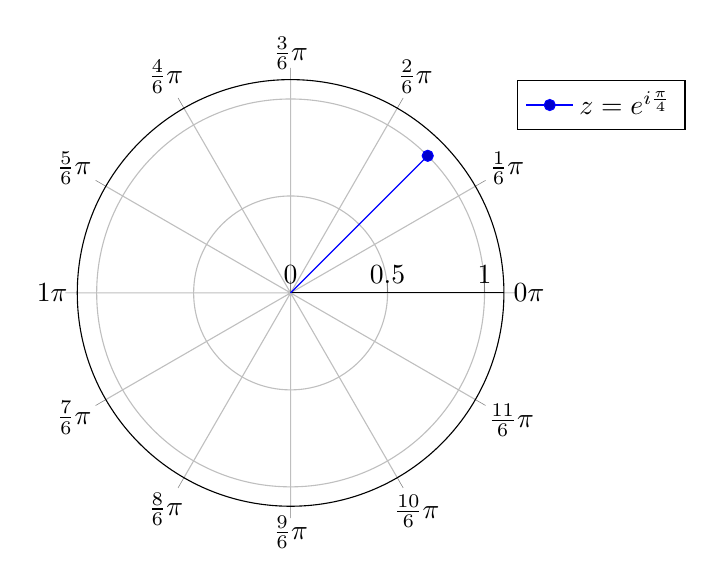
\begin{tikzpicture}
        	    \begin{polaraxis}[xticklabel={
        	    	\pgfmathparse{\tick/180}
        	    	\pgfmathifisint{\pgfmathresult}{$\pgfmathprintnumber[int detect]{\pgfmathresult}\pi$}%
        	    	{$\pgfmathprintnumber[frac,frac denom=6,frac whole=false]{\pgfmathresult}\pi$}
        	    }, legend pos=outer north east]
        	    \addplot+[polar comb] coordinates {(45,1)}; % For future reference: add ordered pairs (degree angle, length) separated by a space (e.g. {(45,1) (90,1) (180,1)})
        	    \legend{$z=e^{i\frac{\pi}{4}}$}
        	    \end{polaraxis}
        	\end{tikzpicture}
        	\caption{Polar representation}
        \end{figure}
    
    \subsection{Definitions of Terms}
        \noindent \textbf{arg$(z)$}: Argument of $z$, also known as $\theta$, $\arg{z}=\arctan{\frac{y}{x}}$ \\*
    
        \noindent \textbf{cis$(\theta)$}: Short-hand for $\cos{\theta}+i\sin{\theta}$ \\*
        
        \noindent \textbf{Complex Conjugate}: Written as $\bar{z}$ it is the reflection about the $Re$ axis (i.e. $z=x+iy \implies \bar{z}=x-iy$) \\*
        
        \noindent \textbf{Im$(z)$}: The imaginary part of $z$ (i.e. the $y$ term)
        
        \noindent \textbf{Magnitude}: Distance from the origin, represented as the radius $r$ (in polar coordinates) and $\left|z\right|=\sqrt{x^2+y^2}$ (in Cartesian coordinates) \\*
        
        \noindent \textbf{Re$(z)$}: The real part of $z$ (i.e. the $x$ term)
        
        
\section{Algebra with Complex Numbers}
    \subsection{Addition}
    	\noindent Addition of complex numbers is done by adding the real parts and imaginary parts: $z_1 + z_2 = (x_1+y_2i)+(x_2+y_2i) = (x_1+x_2)+i(y_1+y_2)$ This can be visualized in the same way as vector addition ("tip-to-tail" method). \\*  
        \begin{figure}[!h]
        	\centering
    	    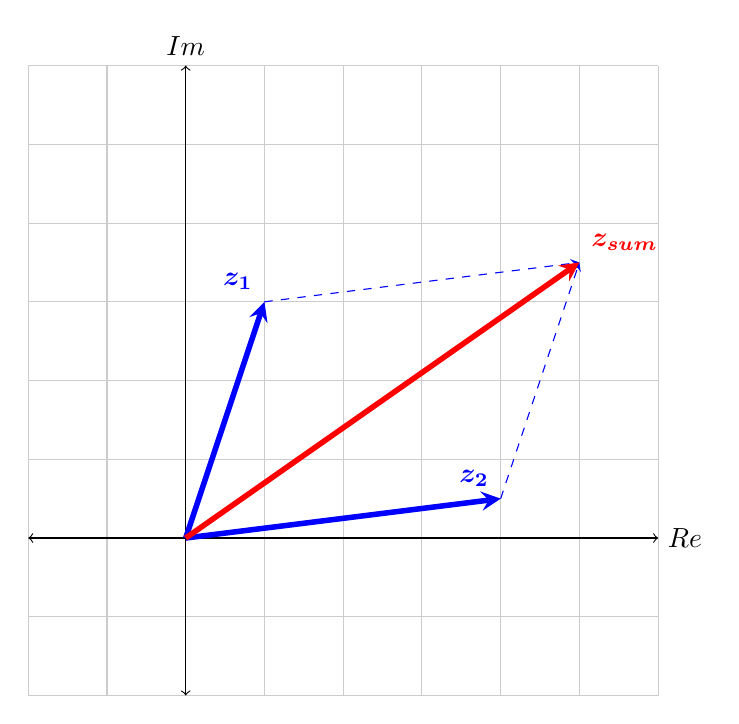
\begin{tikzpicture}
    	        % Axes/grids
    	        \draw[thin,gray!40] (-2,-2) grid (6,6);
         	    \draw[<->] (-2,0)--(6,0) node[right]{$Re$};
    	        \draw[<->] (0,-2)--(0,6) node[above]{$Im$};
    	        % z1
    	        \draw[line width=2pt,blue,-stealth](0,0)--(1,3) node[anchor=south east]{$\boldsymbol{z_1}$};
    	        % z2
    	        \draw[line width=2pt,blue,-stealth](0,0)--(4,0.5) node[anchor=south east]{$\boldsymbol{z_2}$};
    	        % Translated z1
    	        \draw[dashed,blue,-stealth](4,0.5)--(5,3.5);
    	        % Translated z2
    	        \draw[dashed,blue,-stealth](1,3)--(5,3.5);
    	        % Resulant
    	        \draw[line width=2pt,red,-stealth](0,0)--(5,3.5) node[anchor=south west]{$\boldsymbol{z_{sum}}$};
    	    \end{tikzpicture}
        	\caption{The sum $\vec{z_1}+\vec{z_2}$ is the diagonal through the parallelogram formed by $z_1$ and $z_2$}
        \end{figure}
    \subsection{Subtraction}
        \noindent Subtraction of complex numbers is done by adding the real parts and imaginary parts of $z_1$ and $-z_2$: $z_1 - z_2 = (x_1+y_2i)-(x_2+y_2i) = (x_1+y_2i)+(-x_2-y_2i)=(x_1-x_2)+i(y_1-y_2)$ This can be visualized in the same way as vector subtraction ("triangle" method). \\*  
        \begin{figure}[!h]
    	    \centering
    	    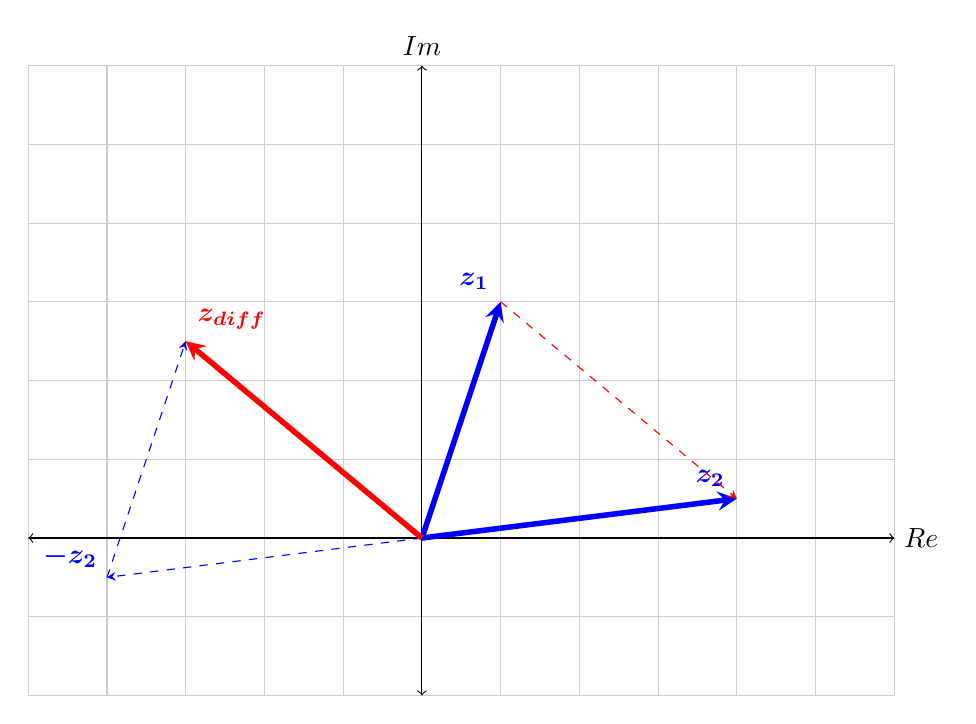
\begin{tikzpicture}
    	        % Axes/grids
    	        \draw[thin,gray!40] (-5,-2) grid (6,6);
    	        \draw[<->] (-5,0)--(6,0) node[right]{$Re$};
    	        \draw[<->] (0,-2)--(0,6) node[above]{$Im$};
    	        % z1
    	        \draw[line width=2pt,blue,-stealth](0,0)--(1,3) node[anchor=south east]{$\boldsymbol{z_1}$};
    	        % z2
    	        \draw[line width=2pt,blue,-stealth](0,0)--(4,0.5) node[anchor=south east]{$\boldsymbol{z_2}$};
    	        % -z2
    	        \draw[dashed,blue,-stealth](0,0)--(-4,-0.5) node[anchor=south east]{$\boldsymbol{-z_2}$};
    	        % Translated z1
    	        \draw[dashed,blue,-stealth](-4,-0.5)--(-3,2.5);
    	        % Resulant
    	        \draw[line width=2pt,red,-stealth](0,0)--(-3,2.5) node[anchor=south west]{$\boldsymbol{z_{diff}}$};
    	        % Translated Resultant
    	        \draw[dashed,red,-stealth](1,3)--(4,0.5);
    	    \end{tikzpicture}
    	    \caption{The difference $\vec{z_1}-\vec{z_2}$ is the third side of the triangle formed by $z_1$ and $-z_2$}
    \end{figure}
    \subsection{Multiplication}
    \subsection{Division}
        
\section{Topological Properties of the Complex Plane}
    \subsection{Definitions}
    \subsection{Weierstrass M-Test}
    \subsection{Stereographic Projection}
\end{document}          
